\section{Removing trivial blocks}

A \textit{trivial block} is defined as a block which is not the first block (having \code{id} equal to \code{0}) and
contains only an \code{UnconditionalJumpStatement}. These blocks can be removed be making the incoming blocks jump
directly to the block to which the trivial block jumps. A trivial block can appear, for example, when the last statement
in the body of a loop is an \code{if} statement. Thus the \code{mergeBlock} of the \code{if} statement contains only an
\code{UnconditionalJumpStatement} to the \code{actualUpdateBlock}.

An example of this pass is provided in \labelindexref{Figure}{img:remove}. The block with \code{id} equal to
\code{6} is trivial and it gets removed by making the incoming blocks (with ids \code{7} and \code{5}) jump directly to
the block to which the trivial block jumps, namely the block with \code{id} equal to \code{1}. The blocks with
\code{id}s \code{1} and \code{6} cannot be inlined because they both have two incoming blocks and the block with
\code{id} \code{7} cannot be inlined either because it is a block appearing after a recursive call.

\begin{figure}[htb]
    \centering
    \begin{subfigure}[b]{\textwidth}
        \centering
        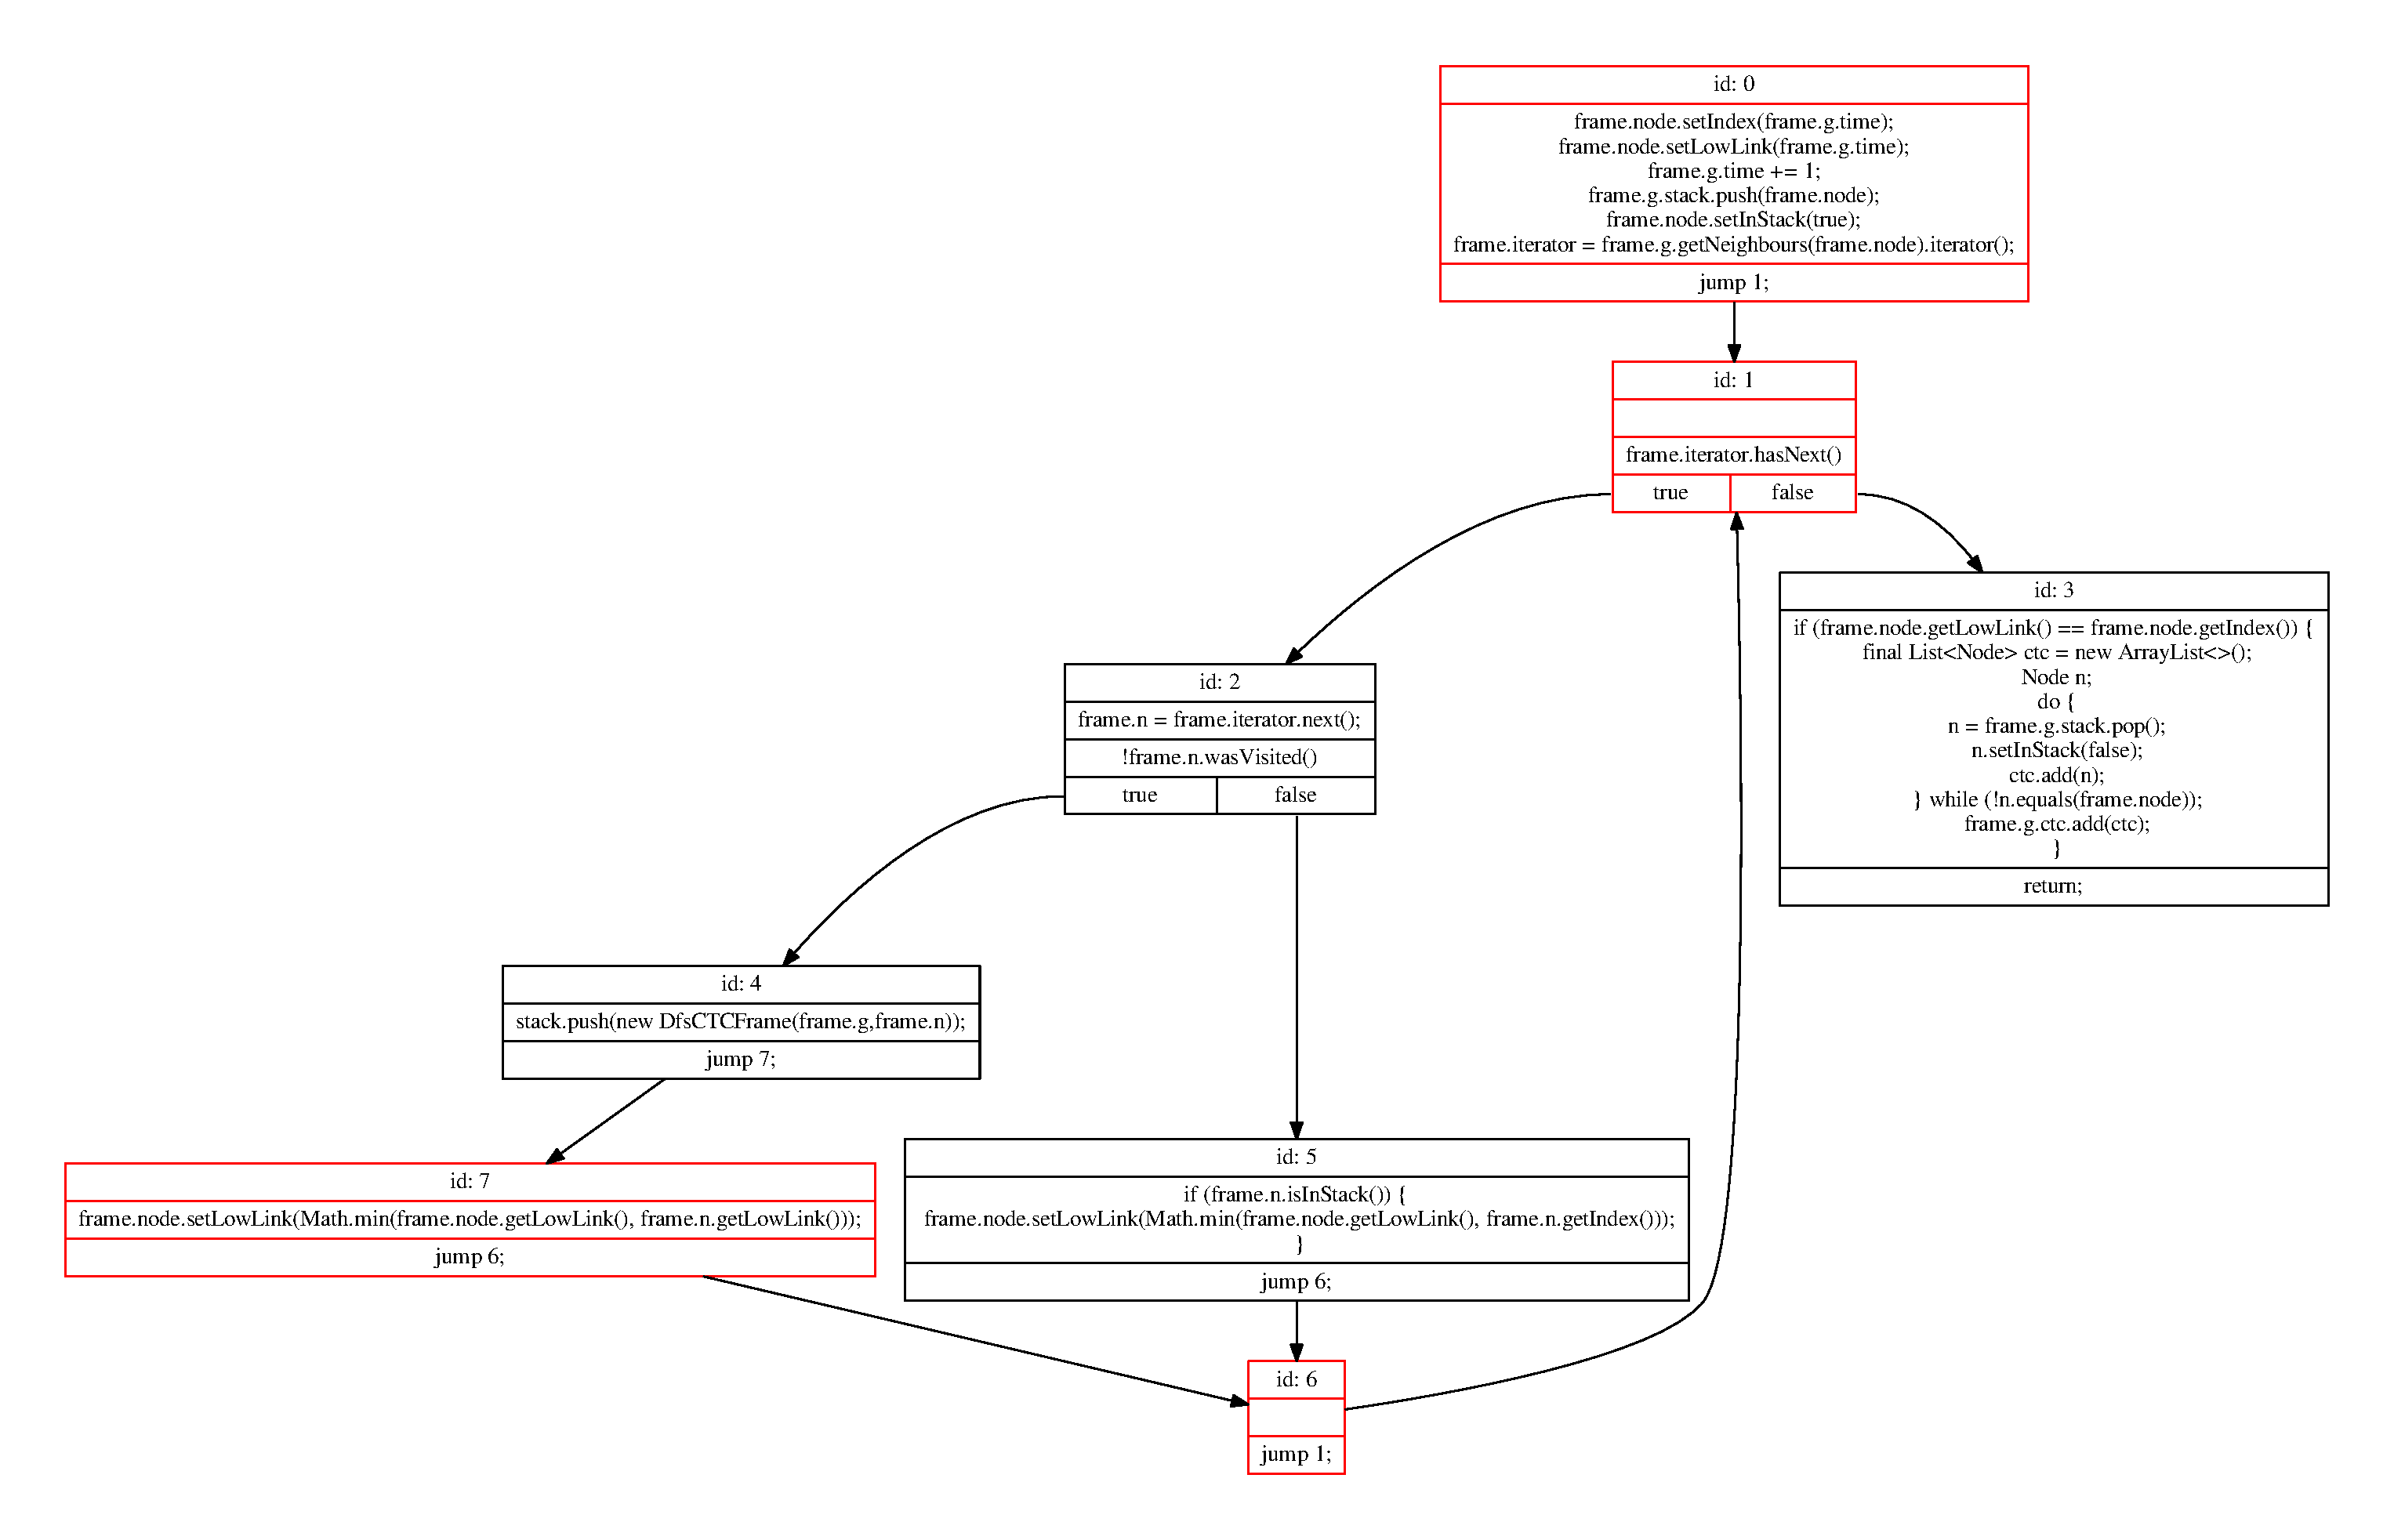
\includegraphics[width=\linewidth]{src/graph/trivial-before.pdf}
        \caption{Before}
    \end{subfigure}
    \begin{subfigure}[b]{\textwidth}
        \centering
        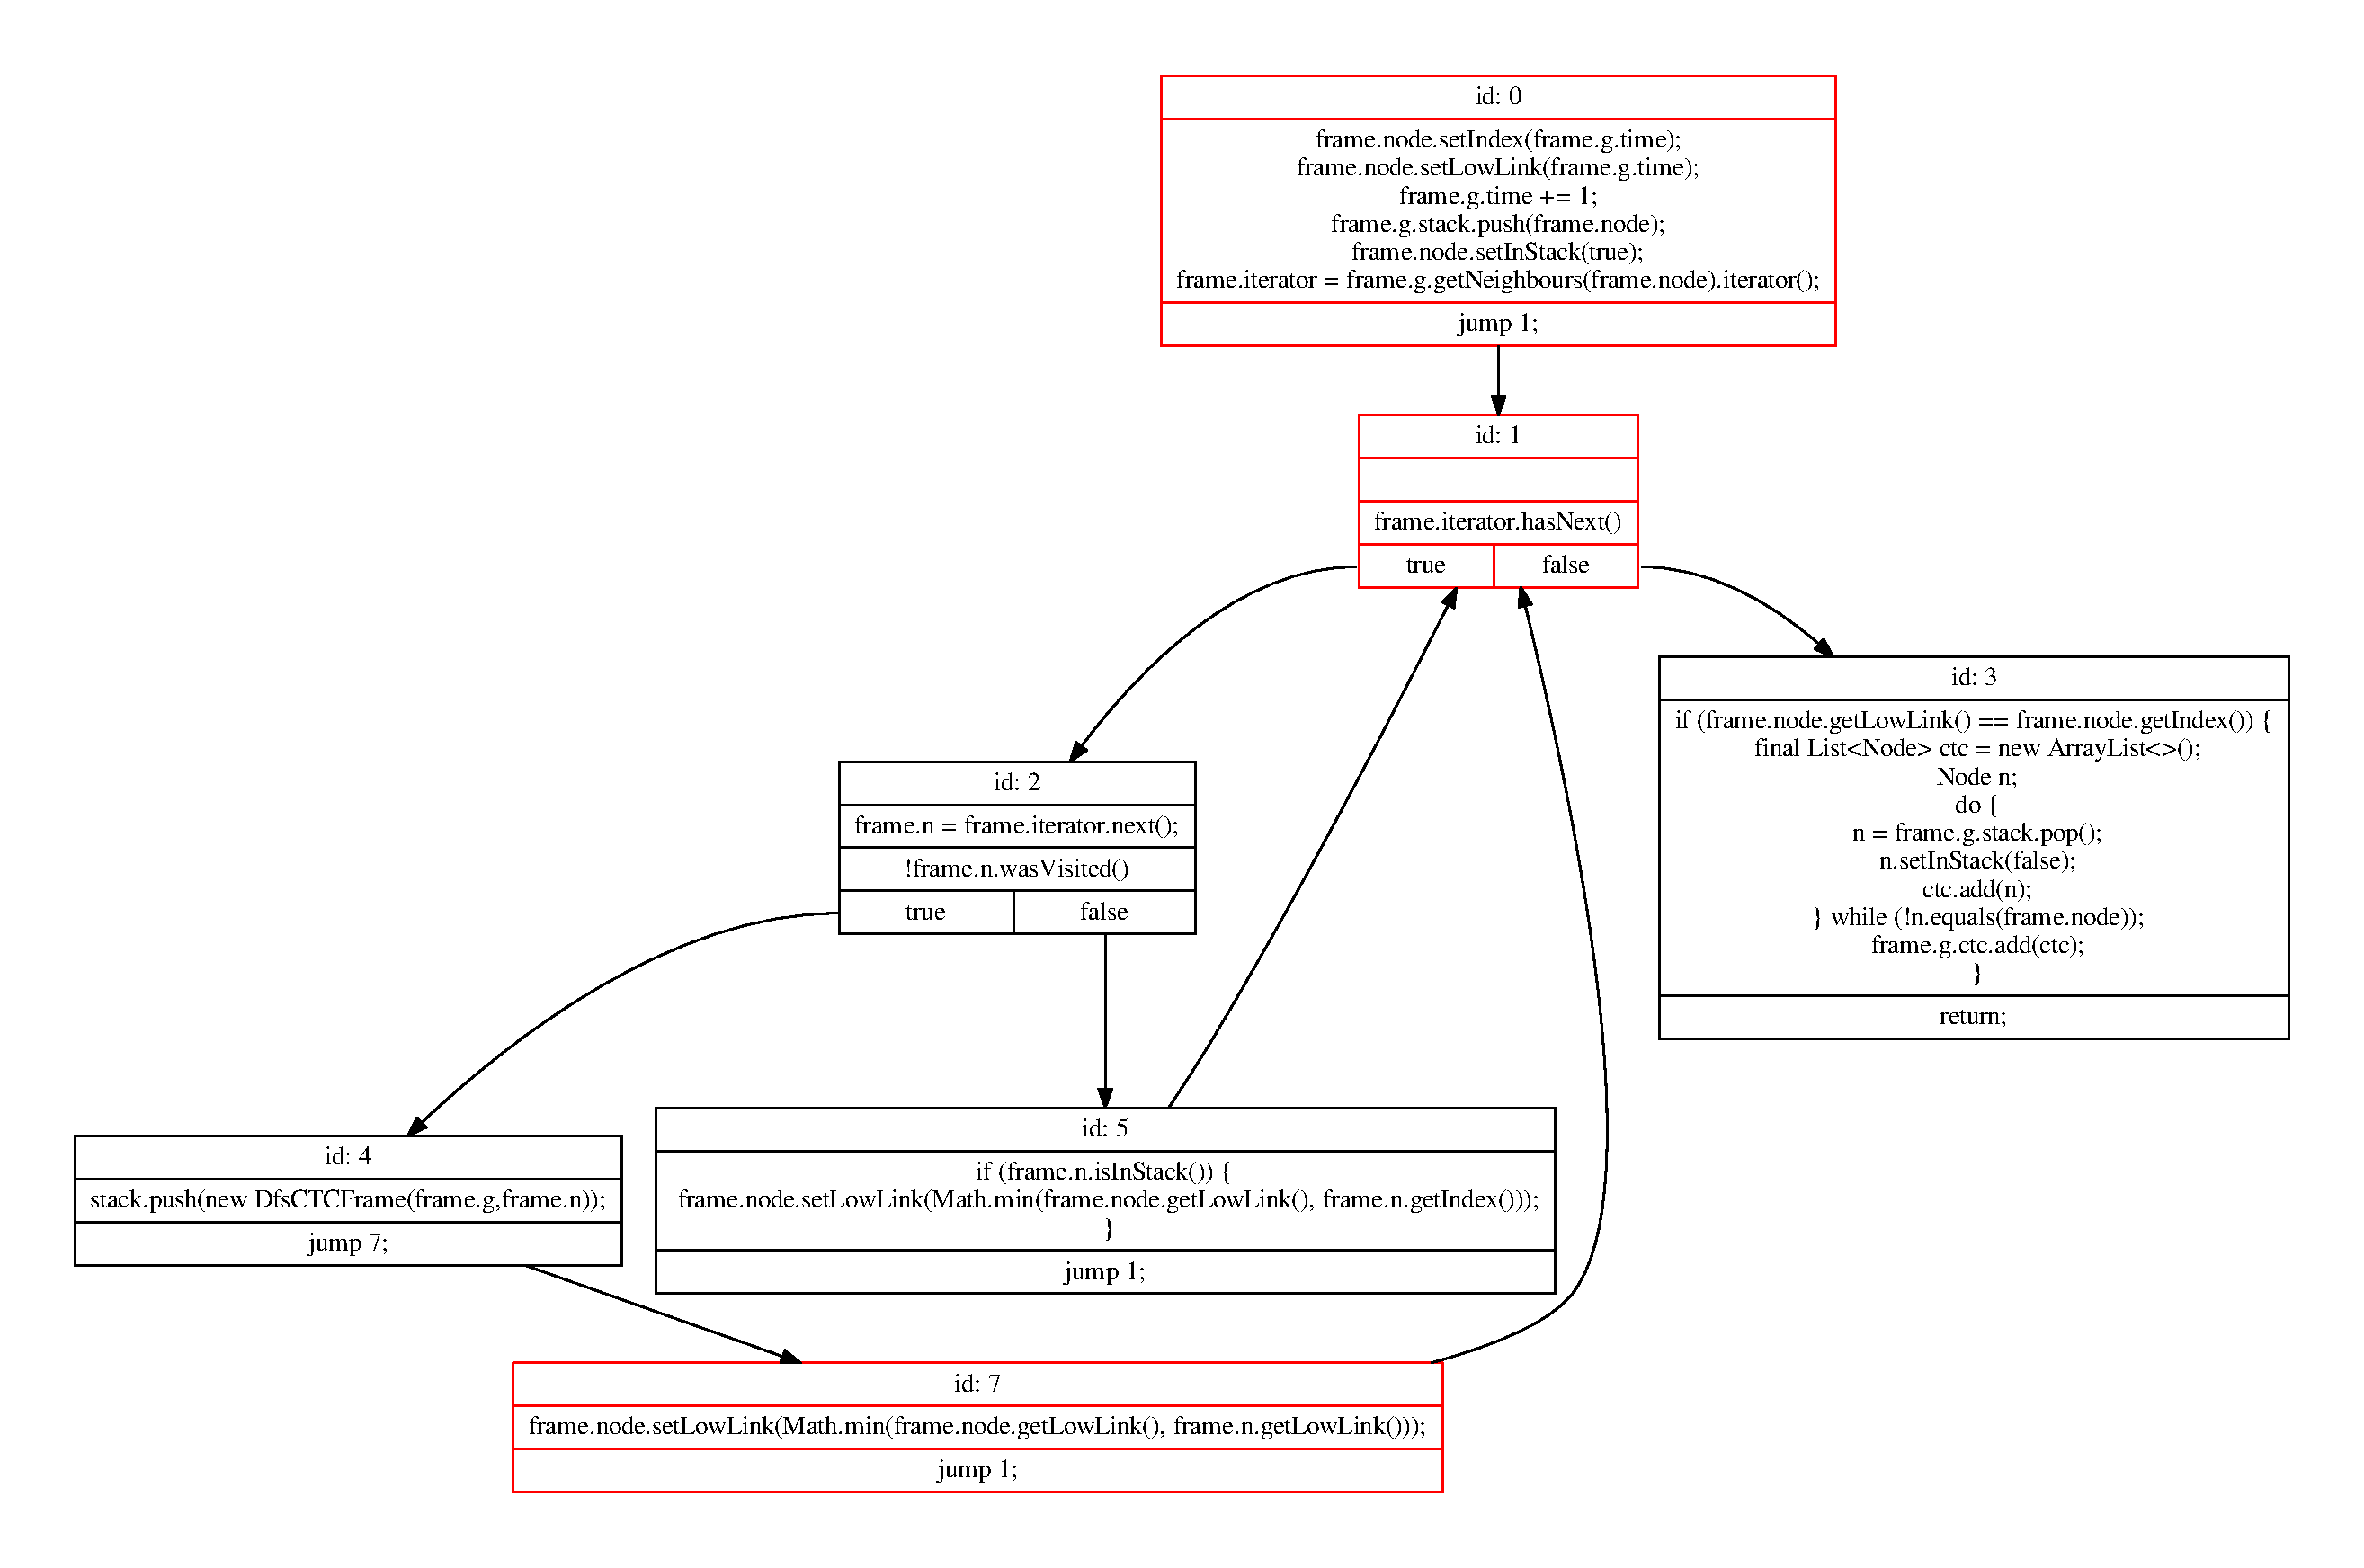
\includegraphics[width=\linewidth]{src/graph/trivial-after.pdf}
        \caption{After \label{img:trivial-after}}
    \end{subfigure}
    \caption{Removing trivial blocks\label{img:remove}}
\end{figure}